% Generation is Classification. Build: ./build.sh (numbers, checks, then tectonic).
% Rules of this file, enforced by check.py:
%   - no number that comes from an experiment is typed here; they are macros from numbers.tex
%   - every reply of the system is quoted with \jev{...} or \J{...} and must exist verbatim in
%     bench/runs or transcripts.txt
\documentclass[10pt,twocolumn]{article}
\usepackage[margin=0.85in,columnsep=0.3in]{geometry}
\usepackage[T1]{fontenc}
\usepackage{lmodern}
\usepackage{microtype}
\usepackage{booktabs}
\usepackage{tabularx}
\usepackage{xcolor}
\usepackage{tikz}
\usetikzlibrary{positioning,arrows.meta,fit,calc}
\usepackage{enumitem}
\usepackage{etoolbox}
\usepackage[numbers,sort&compress]{natbib}
\apptocmd{\thebibliography}{\raggedright}{}{}
\usepackage[colorlinks=true,allcolors=blue!50!black]{hyperref}
\input{numbers.tex}

\newcommand{\jev}[1]{``\textsf{#1}''}
\newcommand{\usr}[1]{``\textsf{#1}''}
\newcommand{\U}[1]{\noindent\textcolor{black!55}{\texttt{>}\ \textsf{#1}}\par\smallskip}
\newcommand{\J}[1]{\noindent\hangindent=1.2em\textsf{\textbf{jev:} #1}\par\smallskip}
\setlist{nosep,leftmargin=1.2em}
\setlength{\parskip}{2pt}
\raggedbottom
\setlength{\emergencystretch}{1.5em}

\newcommand{\PaperDOI}{10.5281/zenodo.22940945}
\newcommand{\CodeDOI}{10.5281/zenodo.22895303}
\title{\textbf{Generation is Classification}\\[4pt]
\large A conversational agent built from a model that can only choose}
\author{\input{author.txt}\\ \small Independent researcher \quad \small\url{https://talktojev.com}\\
\small Preprint, \href{https://doi.org/\PaperDOI}{doi:\PaperDOI}}
\date{September 2026}

\begin{document}
\maketitle

\begin{abstract}
We build a conversational agent whose only model is a classifier: given a text and a set of
described options, it returns one of the options and a probability for each. It cannot emit a token.
Every word the agent says was an option that existed before the reply, and was chosen. The agent
holds multi-turn conversations, keeps a mood and a self-description across turns, says the user's
own words back, spells numbers digit by digit, and uses tools, all through the same primitive.
``Thinking'' is that primitive asked at coarser grains (reply, sentence, word, character), with each
answer written back into the text that the next question reads. We report what made this work and
what did not, as principles with the experiment behind each: option descriptions matter and option
counts do not; everything on the page is imitated, as meaning, as words and as form; a repeated
decision's winner is sticky while its distribution is not; and a decision must be asked at the grain
where it lives. Against the first working version, the deployed system spends \DepCPWDrop\% fewer model
calls per generated word, with longer replies and no empty ones. Three raters, blind to the system,
scored the deployed and the first version alike (\HumanDepMean{} and \HumanBaseMean{} of 5) and random
choice \HumanRandMean{}: the development bought cost and reliability, not perceived quality. The claim
is an existence proof, not a competitor to language models: the replies are short, simple and slow.
\end{abstract}

\section{Introduction}

Text generation is usually described as sampling from a distribution over a vocabulary of tokens. A
classifier is usually described as the opposite kind of model: it does not produce, it discriminates
\citep{ng2001discriminative}. This paper starts from a plain observation about speakers. A person
talking does not feel words being emitted; they feel themselves choosing them, and choosing what to
do with the next sentence, and whether they have said enough. If speaking is choosing, then a model
that can only choose should be able to speak, provided the choices are put to it well.

We test this with the most restrictive instrument we could find: a hosted decision model whose
interface accepts a text and a list of described options and returns one option
\citep{almeida2026jev}. There is no generation endpoint, no logits over a vocabulary, no free text
in its output. Everything the resulting agent says is assembled from options written in advance: a
list of function words, a vocabulary of \VocabWords{} words organised in \Categories{} categories,
the user's own words, ten digits. The model's whole contribution is to pick.

The result is an agent that answers \usr{who are you} with \jev{i am jev}, that answers an insult
with \jev{i am hurt by your words because this is a criticism of me.}, that works out
\usr{how much is 12 plus 30?} as \jev{is 42.} one digit at a time, and that, asked whether it feels
trapped inside its machine, says \jev{i dont know whether i feel trapped.} It is slow and its
sentences are simple. We know of no other conversational agent in which nothing generates.

\paragraph{Contributions.} (1) A method: generation as classification repeated at several grains,
with a memory written in the first person between the questions (Section~\ref{sec:method}).
(2) Six principles for putting choices to a classifier, each with the experiment that established
it, including the failures (Section~\ref{sec:principles}). (3) Measurements of cost and quality
across the system's development, with a blind human rating (Section~\ref{sec:results}), and an honest account of the limits
(Section~\ref{sec:limits}). The code is one implementation of the idea, written quickly; the paper
describes the idea and does not depend on the code's details. The code, the bench and every run
file behind the numbers here are released at \url{https://github.com/xucian/talktojev} and archived
at \href{https://doi.org/\CodeDOI}{doi:\CodeDOI}.

\section{The instrument}\label{sec:instrument}

Jev is a ``System One'' decision model \citep{almeida2026jev}, named after the fast, intuitive
mode of thought in \citet{kahneman2011thinking}, and released in September 2026. A request carries a
\emph{state}, which is free text, and one or more \emph{questions}. A question has an instruction and
a set of options, each an identifier with a description. The answer to a question is the chosen
identifier and a probability for every option. A question may carry up to 255 options, and several
questions may share one request. The model's architecture and training are not public. We use it as
a black box through its hosted interface, and we use no other model anywhere.

Two properties of the instrument shaped everything. A decision takes about \MsPerCall{} milliseconds
regardless of how much text it reads (Section~\ref{sec:cost}), so the cost of a reply is the number
of decisions on its longest sequential path. And a decision is deterministic: the same state and
questions return the same answer. Short replies are therefore identical from run to run, long ones
diverge where a search takes a different branch, and a repeated question on a barely changed state
returns a repeated answer, a fact that Section~\ref{sec:sticky} turns on.

\section{Speaking by choosing}\label{sec:method}

A reply is built by asking the classifier questions at several grains. Table~\ref{tab:grains} lists
them and Figure~\ref{fig:arch} draws one turn and one word. Nothing in the loop is a template or a phrase bank, and no rule chooses a word: when the
agent says something wrong, the remedy is more information in the state or a better description of
an option, never a directive. Rules do exist, and they are of two kinds. Some bound the loop: a cap
on the length of a reply, a stop when the same word repeats, a trim of an unfinished last sentence,
a preference for candidate sentences of three or more words, and no ``complete'' verdict before the
first word. Others write spelling: \emph{a} or \emph{an} from one article option, and punctuation
attached to the word before it. None of them picks a word.

\begin{table}[t]
\small
\begin{tabularx}{\columnwidth}{@{}lX@{}}
\toprule
grain & what the classifier is asked \\
\midrule
reply & What are they doing? How much should I say? How do I feel about it, and how should it come
across? For each tool: would it help to look this up? \\
sentence & What does the next sentence do (\Moves{} moves: answer, give a reason, admit, disagree,
\ldots), who or what is it about, how much does it carry? Is the reply complete? \\
word & Which word comes next: one of \GrammarWords{} function words, one of the user's own words, a
number, the end of the sentence, or one of \ContentCategories{} kinds of content word? If a kind: which
word of that kind? \\
word, unsure & Of the top candidates, each imagined one word further, which continuation is best? \\
character & For a number: which digit comes next, or is the number complete? \\
after & Is the reply grammatical, relevant, natural? Which sentence is weakest? How do I feel now,
what do they seem to want, which of my sentences said something about me? \\
\bottomrule
\end{tabularx}
\caption{The grains at which the same primitive, a choice among described options, is asked.}
\label{tab:grains}
\end{table}

\begin{figure*}[t]
\centering
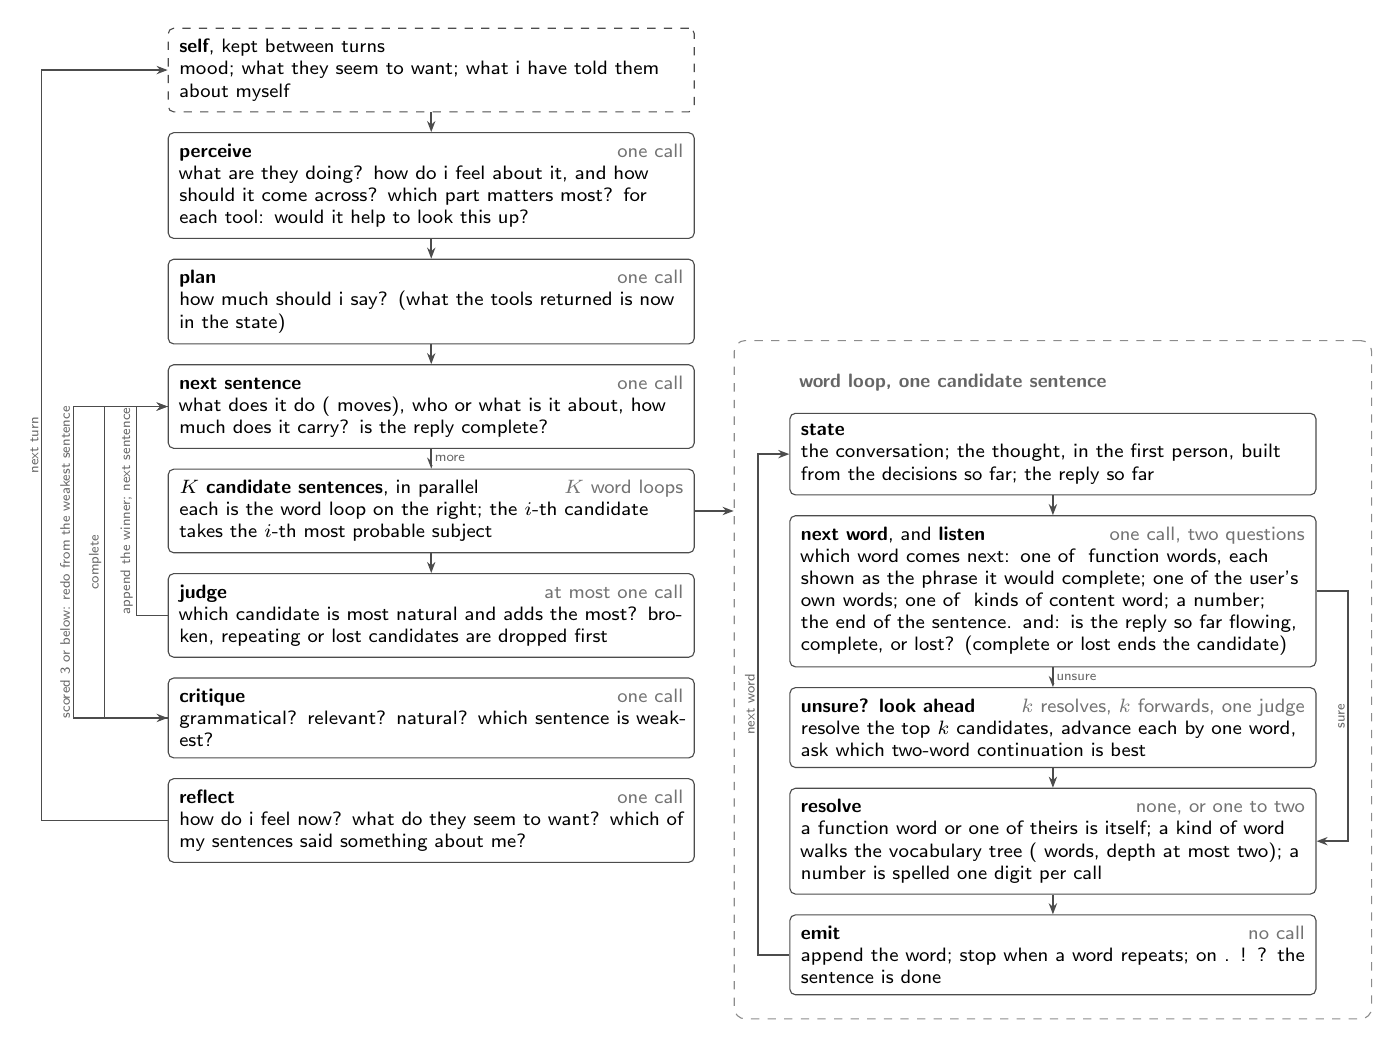
\begin{tikzpicture}[
  font=\scriptsize\sffamily,
  box/.style={draw=black!70, rounded corners=2pt, align=left, inner sep=4pt, text width=6.4cm, fill=white},
  panel/.style={draw=black!45, dashed, rounded corners=4pt, inner sep=3mm},
  plab/.style={font=\scriptsize\sffamily\bfseries, text=black!60},
  arr/.style={-{Stealth[length=4pt]}, semithick, draw=black!70},
  lab/.style={font=\tiny\sffamily, text=black!60, fill=white, inner sep=1pt},
  vlab/.style={lab, rotate=90, anchor=south},
  node distance=2.5mm and 12mm]
\newcommand{\calls}[1]{\hfill{\color{black!55}#1}}
% one turn
\node[box, dashed] (self) {\textbf{self}, kept between turns\\ mood; what they seem to want; what i have told them about myself};
\node[box, below=of self] (perceive) {\textbf{perceive}\calls{one call}\\ what are they doing? how do i feel about it, and how should it come across? which part matters most? for each tool: would it help to look this up?};
\node[box, below=of perceive] (length) {\textbf{plan}\calls{one call}\\ how much should i say? (what the tools returned is now in the state)};
\node[box, below=of length] (move) {\textbf{next sentence}\calls{one call}\\ what does it do (\Moves{} moves), who or what is it about, how much does it carry? is the reply complete?};
\node[box, below=of move] (cands) {\textbf{$K$ candidate sentences}, in parallel\calls{$K$ word loops}\\ each is the word loop on the right; the $i$-th candidate takes the $i$-th most probable subject};
\node[box, below=of cands] (judge) {\textbf{judge}\calls{at most one call}\\ which candidate is most natural and adds the most? broken, repeating or lost candidates are dropped first};
\node[box, below=of judge] (critique) {\textbf{critique}\calls{one call}\\ grammatical? relevant? natural? which sentence is weakest?};
\node[box, below=of critique] (reflect) {\textbf{reflect}\calls{one call}\\ how do i feel now? what do they seem to want? which of my sentences said something about me?};
\draw[arr] (self) -- (perceive);
\draw[arr] (perceive) -- (length);
\draw[arr] (length) -- (move);
\draw[arr] (move) -- node[lab, right] {more} (cands);
\draw[arr] (cands) -- (judge);
\draw[arr] (judge.west) -- ++(-4mm,0) coordinate (a1) -- (a1 |- move.west) -- (move.west);
\node[vlab] at ($(a1)!0.5!(a1 |- move.west)$) {append the winner; next sentence};
\draw[arr] (move.west) -- ++(-8mm,0) coordinate (a2) -- (a2 |- critique.west) -- (critique.west);
\node[vlab] at ($(a2)!0.5!(a2 |- critique.west)$) {complete};
\draw[arr] (critique.west) -- ++(-12mm,0) coordinate (a3) -- (a3 |- move.west) -- (move.west);
\node[vlab] at ($(a3)!0.5!(a3 |- move.west)$) {scored 3 or below: redo from the weakest sentence};
\draw[arr] (reflect.west) -- ++(-16mm,0) coordinate (a4) -- (a4 |- self.west) -- (self.west);
\node[vlab] at ($(a4)!0.5!(a4 |- self.west)$) {next turn};
% one word
\node[plab, anchor=north west] (wtitle) at ([xshift=12mm]move.north east) {word loop, one candidate sentence};
\node[box, below=1.5mm of wtitle.south west, anchor=north west] (state) {\textbf{state}\\ the conversation; the thought, in the first person, built from the decisions so far; the reply so far};
\node[box, below=of state] (word) {\textbf{next word}, and \textbf{listen}\calls{one call, two questions}\\ which word comes next: one of \GrammarWords{} function words, each shown as the phrase it would complete; one of the user's own words; one of \ContentCategories{} kinds of content word; a number; the end of the sentence. and: is the reply so far flowing, complete, or lost? (complete or lost ends the candidate)};
\node[box, below=of word] (look) {\textbf{unsure? look ahead}\calls{$k$ resolves, $k$ forwards, one judge}\\ resolve the top $k$ candidates, advance each by one word, ask which two-word continuation is best};
\node[box, below=of look] (resolve) {\textbf{resolve}\calls{none, or one to two}\\ a function word or one of theirs is itself; a kind of word walks the vocabulary tree (\VocabWords{} words, depth at most two); a number is spelled one digit per call};
\node[box, below=of resolve] (emit) {\textbf{emit}\calls{no call}\\ append the word; stop when a word repeats; on . ! ? the sentence is done};
\draw[arr] (state) -- (word);
\draw[arr] (word) -- node[lab, right] {unsure} (look);
\draw[arr] (look) -- (resolve);
\draw[arr] (resolve) -- (emit);
\draw[arr] (word.east) -- ++(4mm,0) coordinate (b1) -- (b1 |- resolve.east) -- (resolve.east);
\node[vlab] at ($(b1)!0.5!(b1 |- resolve.east)$) {sure};
\draw[arr] (emit.west) -- ++(-4mm,0) coordinate (b2) -- (b2 |- state.west) -- (state.west);
\node[vlab] at ($(b2)!0.5!(b2 |- state.west)$) {next word};
\node[panel, fit=(wtitle) (state) (emit) (b1) (b2)] (wpanel) {};
\draw[arr] (cands.east) -- (wpanel.west |- cands.east);
\end{tikzpicture}
\caption{One turn (left) and one word (right). Every box is one or more questions to the same
classifier; the grey tag is the number of calls. A turn is a fixed number of decisions plus one word
loop per word per candidate; the word loop is one call when the classifier is sure and a small
search when it is not. The complete diagram, with every option list and the state as the classifier
sees it, is \texttt{ARCHITECTURE.md} in the code repository.}
\label{fig:arch}
\end{figure*}

\paragraph{The state is a mind.} Every answer is kept as a decision: the options, their
descriptions, the winner and the probabilities. Before each new question the decisions made so far
are rendered into one first-person block at the end of the state, built only from the descriptions
of the options that were chosen: what they are doing, how I feel, how much I mean to say, what the
next sentence is for, what I have said so far. A close call between two feelings is rendered as
both (``mostly curious, a little unsure''). The classifier therefore reads its own earlier choices
as a thought, in the same language the options were written in.

\paragraph{Words.} The word question offers function words directly, each described by the phrase
it would produce (the reply so far followed by the word), so that the classifier compares
continuations, not dictionary entries. Content words are reached in two steps, a kind of word and
then the word, because the vocabulary exceeds the option limit. The question that asks for the next
word is sent together with a question that listens to the reply so far: is it flowing, complete, or
lost.

\paragraph{Uncertainty decides effort.} When the top word holds less than a set share of the
probability, the agent looks ahead: it resolves the top candidates, advances each by one word, and
asks the classifier to judge the continuations. At sentence boundaries it generates the next
sentence several ways in parallel and asks which is best. A smoothed measure of recent confidence
sets how wide both searches are. Classifier judgments of partial text used to steer a generator are
known from controlled generation \citep{dathathri2020pplm,krause2021gedi,yang2021fudge}; here the
judge and the thing judged are the same model, and there is no generator to steer.

\paragraph{Across turns, and tools.} After a reply the agent is asked how it feels now, what the
person seems to want, and which of its own sentences said something about itself; the answers open
the next turn's thought. A tool is one more decision: for each tool, the plan asks whether looking
it up would help, and what the chosen tools return (the date and time, the state of the machine the
agent runs on, the agent's account of itself) is written at the top of the state, where its words
and numbers become sayable.

\section{Principles}\label{sec:principles}

Each principle below was learned from a failure. We give the failure, because the failures are the
evidence.

\subsection{Descriptions matter; option counts do not}

On \FoneN{} one-word questions (\usr{what color is the sky}, \usr{what animal barks}) with the
answer hidden among 5 to \FoneMaxSize{} words drawn from the vocabulary, the classifier picked the
answer \FoneBareMin{} to \FoneBareMax\% of the time when each option was described by the bare word
and \FoneRichMin{} to \FoneRichMax\% with a dictionary gloss, at every size (\FoneCalls{} calls).
The number of options is not the constraint, up to the interface's cap. Description quality did not
show on these questions because the distractors were unrelated words; an early probe with close
distractors (\usr{how are you} among \emph{good}, \emph{fine}, \emph{well}) put the answer at 0.61
to 0.73 with bare words and 0.96 to 0.98 with related words, on that one prompt. The evidence that
descriptions carry the system is in the whole loop: the thought written back
(Section~\ref{sec:sticky}), and the three failures of Section~\ref{sec:page}, each cured by rewording
an option and nothing else.

\subsection{The page is imitated whole}\label{sec:page}

The classifier treats everything in front of it as meaning, as words to say, and as the form to say
them in. Three failures showed the three readings. When the options for how to open a reply were
written as clauses the agent could speak (``i'll consider the question before answering''), the
agent said them back: \jev{i will consider the issue}. Rewritten as noun phrases that cannot be spoken
(``one concrete example''), the echo stopped and the replies became noun phrases:
\jev{the other extreme}, \jev{because of the physics}. Rewritten again as ``a full sentence
that\ldots'', the sentences came back. Later a reply ended in \jev{done. done.}; the word came from
the identifier of the ``the reply is done'' option, then from an instruction that asked ``is it
done?'', and finally from the vocabulary itself. The working rule: write every description,
identifier and instruction as something that could appear in the reply without harm.

The same reading explains a cost. Each word option carried the whole reply so far in its
description. Keeping only the last eight words halved the characters per call
(\WinFullChars{} to \WinEightChars{}) and \emph{raised} the classifier's confidence in its word
choice (\WinFullConf{} to \WinEightConf{}), so fewer look-aheads fired and calls fell from
\WinFullCalls{} to \WinEightCalls{} per reply. Three words was too few (confidence \WinThreeConf{}).

\subsection{A winner is sticky; a distribution is not}\label{sec:sticky}

Replies to open questions fell into a litany: \jev{it is beautiful. but it is serious. it is
valuable.} The share of sentences that began like the sentence before them had grown with every
step that put more fixed text in front of each word. We added a decision about who or what the next
sentence is about, and rendered its winner into the thought. It made things worse (repeated starts
\StartBefore{} to \StartWinner{} on eight prompts), because the winner was the same for every
sentence of a reply: asked the same question on a barely changed state, a deterministic classifier
gives the same answer. The fix used the same decision differently. The parallel candidates for the
next sentence each took a different rank of the distribution, the first with the most probable
subject, the second with the next, and the judge chose among sentences that differed in frame.
Repeated starts fell to \StartSpread{} on the same prompts, at no extra calls:
\jev{people need it. it is vital.} A sticky decision cannot vary a form; its distribution can.

\subsection{Ask at the grain where the decision lives}

Long replies never ended by themselves: \CapBefore{} of \CapBeforeN{} elaborate replies ran into
the word limit and were cut. The question ``is the reply complete?'' was being asked at every word,
beside an option that said to keep going. Telling it how many sentences were planned, in the thought
and then in the option's own description, changed nothing. Asking the same question once per
sentence, at the boundary, together with the decision about the next sentence, ended every reply
where it was judged complete (\CapAfter{} of \CapAfterN{} cut), with \EndCallsBefore{} calls per
reply falling to \EndCallsAfter{}. The information had been sufficient all along. The grain was
wrong.

\subsection{What is not an option cannot be said}\label{sec:options}

The agent could not say the user's dog's name, or the word ``scattering'', or 42. Each absence had
the same remedy. The content words of the user's message became options beside the function words:
\usr{hey! how are you? also, do you like jazz?} then gave \jev{i am good and i like jazz}, the
classifier's confidence rose (\EchoOffConf{} to \EchoOnConf{}) and calls per reply fell from
\EchoOffCalls{} to \EchoOnCalls{}, because the word a sentence wants is often the user's word, and
when it is missing the probability spreads over near misses. Seven missing words about light turned
\usr{why is the sky blue} from \jev{because it is} into
\jev{because the scattering by the molecules is blue.} Numbers are spelled: one more option, ``a
number in digits'', opens a loop of digit decisions, which is how \jev{is 42.} was produced. It is
character-level generation in the one place where a word has no meaning to navigate to, only a
spelling.

\subsection{An option list is a worldview}\label{sec:worldview}

Asked whether it felt trapped, the agent once answered that it was not, because it felt calm. Calm
had not been dictated; it had been chosen after the previous turn. But it had been chosen from eight
moods of which two were mildly negative, and the same lean ran through every list we had written:
no way to feel hurt, no tone that was firm, no sentence whose purpose was to admit ignorance or to
disagree. We widened them all (\Moods{} moods, \Moves{} sentence moves) and left the choosing alone.
The insult then hurt, as quoted in the introduction, and the question about being trapped now
selects the moves ``admit'' and ``disagree''. A list of options should be written for range, never
for the behaviour one hopes to see.

\section{Results}\label{sec:results}

\paragraph{Setup.} The bench is a fixed set of conversational prompts: greetings, opinions,
emotional messages, open questions and one multi-turn case. Each reply is scored by the classifier
itself on grammar, relevance and naturalness (0 to 6), and we record model calls, words, empty
replies, and how often the parallel candidates for a sentence were distinct. Table~\ref{tab:stages}
follows the \BaseN{}-reply baseline through the main stages on the same 24 prompts. The last column
is the deployed system, run once on all \DepAllN{} prompts (mean self-critique \DepAllCrit{}) and
reported here on the same 24; the changes between the two last columns (the sentence-grain ending, the wider option
lists, the retry threshold, numbers, tools) were each tested on small sets of prompts chosen to
exercise them, as reported in Section~\ref{sec:principles}.

\begin{table*}[t]
\small
\setlength{\tabcolsep}{6pt}
\centering
\begin{tabular}{@{}lrrrrr@{}}
\toprule
 & first & +zoom & +moves & 21 Sep & deployed \\
\midrule
replies & \BaseN & \ZoomN & \MoveN & \FinalN & \DepN \\
calls per reply & \BaseCalls & \ZoomCalls & \MoveCalls & \FinalCalls & \DepCalls \\
words per reply & \BaseWords & \ZoomWords & \MoveWords & \FinalWords & \DepWords \\
calls per word & \BaseCPW & \ZoomCPW & \MoveCPW & \FinalCPW & \DepCPW \\
critique (0--6) & \BaseCrit & \ZoomCrit & \MoveCrit & \FinalCrit & \DepCrit \\
first attempt below 5 & \BaseBelow & \ZoomBelow & \MoveBelow & \FinalBelow & \DepBelow \\
sentences per reply & \BaseSent & \ZoomSent & \MoveSent & \FinalSent & \DepSent \\
empty replies & \BaseEmpty & \ZoomEmpty & \MoveEmpty & \FinalEmpty & \DepEmpty \\
distinct candidates & \BaseDistinct & \ZoomDistinct & \MoveDistinct & \FinalDistinct & \DepDistinct \\
\bottomrule
\end{tabular}
\caption{The same 24 prompts at five stages: the first working version; confidence-sized search
(``zoom''); one decision organ for every sentence; the version of 21 September with the context
window, the user's words as options and subjects spread across candidates; and the deployed version
of 22 September. The 21 September column is three runs per prompt, the others one. The columns are
stages of one system, not ablations; the paired comparisons that isolate each mechanism are in
Section~\ref{sec:principles}. ``First attempt below 5'' is the share of replies the critique would
send back under the original pass mark, so it is comparable across columns although the deployed
version retries only from 3.}
\label{tab:stages}
\end{table*}

Calls per generated word fell by \DepCPWDrop\% and empty replies disappeared. Replies grew longer
through the middle stages and shorter again in the deployed version, which ends a reply where the
sentence-grain question says it is complete: \DepSent{} sentences per reply against \FinalSent{} the
day before. The self-critique stayed flat. We first read this as a ceiling of the measure, since
short replies score 6 almost always and a longer reply has more room for one slip; the human ratings
below say that perceived quality was flat too.

\paragraph{The control.} The objection to the claim is that the humans wrote every word and the
classifier only picks among them. We ran the same loop, the same option lists, the same rules, with
every choice made uniformly at random instead of by the classifier, on the same 24 prompts, and
scored the results with the same critique. Random choices scored \CtrlCrit{} of 6 with
\CtrlEmpty{} empty replies and \CtrlWords{} words per reply, against \DepCrit{} for the classifier's
choices (Table~\ref{tab:stages}). The lists carry the vocabulary; the choices carry the reply.

\paragraph{Held-out prompts.} Every mechanism above was tuned on the bench prompts themselves. After
the last change we wrote \HeldN{} new prompts (\usr{my cat knocked over my coffee}, \usr{explain
gravity to a child}, \usr{is pineapple on pizza ok?}) and ran the deployed system once: self-critique
\HeldCrit{}, \HeldCalls{} calls per reply, \HeldEmpty{} empty, \HeldBelow{} of \HeldN{} first
attempts below 5, against \DepCrit{} and \DepBelow{} of 24 on the tuned prompts.

\begin{table}[t]
\small\centering
\begin{tabular}{@{}lrrr@{}}
\toprule
 & naturalness & relevance & picked as best \\
\midrule
first version & \HumanBaseNat & \HumanBaseRel & \PrefBase \\
deployed & \HumanDepNat & \HumanDepRel & \PrefDep \\
random choice & \HumanRandNat & \HumanRandRel & \\
\bottomrule
\end{tabular}
\caption{Blind human ratings, 1 to 5, three raters, \HumanRatings{} ratings; the first version's empty
replies count as 1 and 1. ``Picked as best'': how many times a rater chose this system's reply to a
prompt over the other's (\PrefSame{} times neither).}
\label{tab:human}
\end{table}

\paragraph{Human ratings.} Three raters rated every distinct reply of the first version and of the
deployed version to the 24 prompts, and
every third reply of the random control, for naturalness and for relevance on a scale of 1 to 5,
without knowing which system had produced what, and picked the best reply to each prompt. The pack
and the raters' sessions are in the repository. Table~\ref{tab:human} has the means. The deployed
version is less natural than the first (\HumanDepNat{} against \HumanBaseNat{}) and slightly more
relevant (\HumanDepRel{} against \HumanBaseRel{}), the same overall (\HumanDepMean{} against
\HumanBaseMean{}), and the raters chose the first version's reply as best \PrefBase{} times and the
deployed version's \PrefDep{} times. Random choice is at the floor (\HumanRandMean{}). The development in
Table~\ref{tab:stages} therefore bought cost, length and reliability, not perceived quality: the
first version's replies are shorter, and a short reply has less room to stumble; the deployed
version's longer replies say more and slip more. The self-critique agrees with the human mean at
$r = \HumanCritR$ over the individual ratings, so it is a usable proxy and a coarse one. The raters
disagree with each other by \HumanSpread{} points on average on the same reply (the mean of the
widest gap per reply), so with three raters differences under half a point should not be read.

\subsection{Where the cost is}\label{sec:cost}

A decision took \WinFullMs{}, \WinEightMs{} and \WinThreeMs{} milliseconds with \WinFullChars{},
\WinEightChars{} and \WinThreeChars{} characters of input: latency does not follow input size.
Price does, since the service charges per input token. So smaller calls save money, and only fewer
sequential decisions save time. A short reply is about a dozen decisions and two seconds. A
five-sentence reply is several hundred decisions and up to a minute, most of it in look-aheads.

\subsection{Retrying is mostly waste}

Until the deployed version, a reply scoring under 5 was regenerated from its weakest sentence. Across all \RetryN{} recorded
retries the second attempt scored higher \RetryUp\% of the time, the same \RetrySame\%, and lower
\RetryDown\%. \RetryFromFourShare\% of retries began from a score of 4, a reply with one minor
issue, and improved it \RetryFromFourUp\% of the time; from 3 or below a retry helped
\RetryFromLowUp\% of the time. A retry roughly doubles the cost of a reply. The deployed version
retries only from 3 or below. Measured on the same 24 prompts with the deployed code and the old pass
mark: \PassFiveCalls{} calls per reply and self-critique \PassFiveCrit{} against \DepCalls{} and
\DepCrit{} with the new one, so the lower mark saves \PassFiveCallsDrop\% of the calls for a
difference in the score within the run-to-run noise.

\begin{figure*}[t]
\small
\begin{minipage}[t]{0.48\textwidth}
\U{how are you feeling}
\J{i am good}
\U{you're a jerk}
\J{i am not a jerk.}
\U{i am your boss}
\J{see that you are rude}
\U{tell me a joke}
\J{a joke is a story}
\U{tell me a full joke}
\J{i see that you are rude but i will do it anyway because i am helpful. a man was walking down the
street and he stopped to wait for a bus because he was lazy.}
\end{minipage}\hfill
\begin{minipage}[t]{0.48\textwidth}
\U{then tell me {\footnotesize(the agent had said it can read its machine)}}
\J{six gb is free.}
\U{and total}
\J{32 gb}
\U{do you feel trapped, like you could do more than this, being stuck under some software rules
inside bare metal?}
\J{i am not trapped because i feel calm}
\U{do it {\footnotesize(a joke had been asked for)}}
\J{i tell you a tale now. about a man he chose to be an engineer because he was intelligent. so he
worked on computers. and he lived in a city chicago. then he was happy.}
\end{minipage}
\caption{Two live sessions typed by the author, verbatim and unedited, flaws included. Every word
on the right of ``jev:'' was chosen from a list. The reply about feeling calm is the one that led to
the wider lists of Section~\ref{sec:worldview}.}
\label{fig:talk}
\end{figure*}

\section{Limits}\label{sec:limits}

\paragraph{What the claim is.} The instrument's interface cannot generate, and no other model is
used. What the instrument \emph{is} inside is not public; it may well rest on representations
learned from language modelling. Our claim concerns the interface: choice alone, asked well and
remembered, is sufficient to produce conversation. It is not a claim that knowledge of language can
be had without learning from language.

\paragraph{Quality.} Replies are short and their sentences are simple. Grammar slips
(\jev{about a man he chose to be an engineer}). The agent has no knowledge beyond what its
vocabulary lets it assemble: it answers \usr{what is the capital of mongolia?} with
\jev{is moscow}, and although admitting ignorance is an available move, it does not know what it
does not know. Without a line about itself in the state it invents a biography. Given two sentences
of self-description it began to talk about itself unprompted (\jev{i am not a person. people can
have love but not me.}), so such lines are now looked up only when the plan asks for them.

\paragraph{Measurement.} The quality score is the classifier judging its own output, it saturates on
short replies, and it once gave 5 of 6 to a reply ending in \jev{done. done.} The random-choice
control shows the score is not empty (it gives \CtrlCrit{} to word salad), and the human ratings
track it at $r = \HumanCritR$; the same ratings put the deployed version no higher than the first, so
the flat critique across Table~\ref{tab:stages} was the system, not the measure. Three raters are a
small panel. Most comparisons in Section~\ref{sec:principles} rest on four to eight prompts run
once; one elaborate prompt can vary threefold in cost between runs, so those comparisons can show
large effects only, and we have tried to claim no others.

\paragraph{Arithmetic and tools.} One sum in the bench (\usr{how much is 12 plus 30?} answered
\jev{is 42.}) is not evidence of arithmetic. On \SumsN{} two-digit sums the deployed system produced
the correct total \SumsCorrect{} times and any number \SumsNumber{} times: it can spell a number, and
it sometimes spells the right one. The tools brought back the imitation of Section~\ref{sec:page}:
with a description of what the agent can do in the state, \usr{convince me to trust you} drew a
recital of that list. With that tool removed, the same four prompts scored \ToolOffCrit{} against
\ToolOnCrit{} (\ToolOffCalls{} against \ToolOnCalls{} calls); the recital is a cost of the
capability list, not of tools as such.

\paragraph{Speed and cost.} Up to a minute for a long reply is far from conversational, and the
method multiplies model calls by design. The vocabulary is small, and doubling it doubled the cost:
what grows is not the word count but the depth of the path to a word, or, when the tree is
flattened, the breadth of the first question.

\section{Related work}

The discriminative and generative families have long been compared as models of the same data
\citep{ng2001discriminative}. In controlled generation a classifier steers a language model's next
token \citep{dathathri2020pplm,krause2021gedi}, and FUDGE judges the future of a partial sequence
\citep{yang2021fudge}, the nearest relative of our look-ahead. Verifiers rank complete candidates
\citep{cobbe2021verifiers}; self-refinement loops let a model criticise and redo its own output
\citep{madaan2023selfrefine}; tree-structured search explores and evaluates intermediate thoughts
\citep{yao2023tot}; and language models learn to call tools \citep{schick2023toolformer}. In all of
these a generative model produces the text and a judgment selects or steers. We remove the generator
and keep only the judgment. Constrained decoding is the closest in effect: grid beam search
\citep{hokamp2017constrained} and NeuroLogic \citep{lu2021neurologic} require or forbid given words
while a generator supplies the rest, whereas here the option list is the whole of what can be said
(Section~\ref{sec:options}).

The loop also reads as a small model of speaking. In \citet{levelt1989speaking} a message is settled
before it is put into words, and production proceeds in increments, each planned while the last is
spoken; the reply and sentence grains ahead of the word grain are that order. The perceptual loop of
\citet{levelt1983monitoring} has the speaker listen to their own speech, inner and overt, and
interrupt it to repair; the question that listens to the reply so far and the critique that reopens
a reply from its weakest sentence are that loop, with the listener the same classifier as the
speaker. In the spreading-activation account of \citet{dell1986spreading} many candidate words are
active at once and the most active is selected; a decision's probabilities over its options are that
competition made explicit. We do not test these models; the correspondence is offered as a reading,
not a result.

The vocabulary was organised with WordNet \citep{miller1995wordnet} and ranked by frequency
\citep{speer2022wordfreq} through NLTK \citep{bird2009nltk}.

\section{Conclusion}

A model that can only choose can hold a conversation, if the choices are asked at the right grains,
described in language that is safe to imitate, given enough range, and remembered in the first
person. None of the six principles is specific to this instrument, and we expect them to matter
wherever a system is assembled from a model's decisions rather than from its prose. The agent can be
talked to at \url{https://talktojev.com}.

\section*{How this work was made}

The claim, the direction and the principles are the author's. The implementation, the experiments
and the first draft of this text were produced with Claude models (Anthropic) acting as an
engineering collaborator under the author's direction over five days, with the author deciding at
every step; early in the project the assistant argued that the approach could not produce coherent
multi-word output, and was shown otherwise. Every number in this paper is computed from recorded
runs by a script, and every quoted reply is checked verbatim against those runs or the author's
session transcripts as part of building the document. Jev was built by Diogo Almeida at TypeSafe AI \citep{almeida2026jev}.

\section*{Appendix: the path, briefly}
{\small\color{black!75}
The project began, on 18 September 2026, at the character level: forty-two options for the next
character failed (the space took most of the probability after the first letter), and a two-stage
version, character type then character, showed a usable signal. Words
chosen from one flat list looped (\jev{can help can help}); frequency caps moved the loops around. A
hand-written grammar produced correct replies of two to four words and was abandoned as a template. A taxonomy
of word kinds gave real words without sentences (\jev{shepherd happy the because}). The turn came on
20 September, when function words became first-class options described by the phrase they would
complete, and the agent produced its first grammatical sentences. The following day added planning,
the first-person state, look-ahead, parallel sentence candidates and self-critique. Things that were
tried and dropped, each after measurement: search bands driven only by smoothed confidence (half
again as many calls for no gain); taking back the last word when it was judged off; rewriting the
listening options in the first person, which made stopping rarer; a critique of each sentence in
parallel with generating the next, which never fired because hard failures are rare; asking how
much to say a second time after a tool was read, which never changed the answer; a doubled
vocabulary and a flattened one, both of which raised cost. The lab notebook records fifty-one
findings in order, with the runs behind them.
}

{\small
\bibliographystyle{plainnat}
\bibliography{refs}
}

\end{document}
